\documentclass{article}
\usepackage{physics}
\usepackage{graphicx}
\usepackage{caption}
\usepackage{amsmath}
\usepackage{bm}
\usepackage{framed}
\usepackage{authblk}
\usepackage{empheq}
\usepackage{amsfonts}
\usepackage{esint}
\usepackage[makeroom]{cancel}
\usepackage{dsfont}
\usepackage{centernot}
\usepackage{mathtools}
\usepackage{subcaption}
\usepackage{bigints}
\usepackage{amsthm}
\theoremstyle{definition}
\newtheorem{lemma}{Lemma}
\newtheorem{defn}{Definition}[section]
\newtheorem{prop}{Proposition}[section]
\newtheorem{rmk}{Remark}[section]
\newtheorem{thm}{Theorem}[section]
\newtheorem{exmp}{Example}[section]
\newtheorem{prob}{Problem}[section]
\newtheorem{sln}{Solution}[section]
\newtheorem*{prob*}{Problem}
\newtheorem{exer}{Exercise}[section]
\newtheorem*{exer*}{Exercise}
\newtheorem*{sln*}{Solution}
\usepackage{empheq}
\usepackage{tensor}
\usepackage{xcolor}
%\definecolor{colby}{rgb}{0.0, 0.0, 0.5}
\definecolor{MIT}{RGB}{163, 31, 52}
\usepackage[pdftex]{hyperref}
%\hypersetup{colorlinks,urlcolor=colby}
\hypersetup{colorlinks,linkcolor={MIT},citecolor={MIT},urlcolor={MIT}}  
\usepackage[left=1in,right=1in,top=1in,bottom=1in]{geometry}

\usepackage{newpxtext,newpxmath}
\newcommand*\widefbox[1]{\fbox{\hspace{2em}#1\hspace{2em}}}

\newcommand{\p}{\partial}
\newcommand{\R}{\mathbb{R}}
\newcommand{\C}{\mathbb{C}}
\newcommand{\lag}{\mathcal{L}}
\newcommand{\nn}{\nonumber}
\newcommand{\ham}{\mathcal{H}}
\newcommand{\M}{\mathcal{M}}
\newcommand{\I}{\mathcal{I}}
\newcommand{\K}{\mathcal{K}}
\newcommand{\F}{\mathcal{F}}
\newcommand{\w}{\omega}
\newcommand{\lam}{\lambda}
\newcommand{\al}{\alpha}
\newcommand{\be}{\beta}
\newcommand{\x}{\xi}

\newcommand{\G}{\mathcal{G}}

\newcommand{\f}[2]{\frac{#1}{#2}}

\newcommand{\ift}{\infty}

\newcommand{\lp}{\left(}
\newcommand{\rp}{\right)}

\newcommand{\lb}{\left[}
\newcommand{\rb}{\right]}

\newcommand{\lc}{\left\{}
\newcommand{\rc}{\right\}}


\newcommand{\V}{\mathbf{V}}
\newcommand{\U}{\mathcal{U}}
\newcommand{\Id}{\mathcal{I}}
\newcommand{\D}{\mathcal{D}}
\newcommand{\Z}{\mathcal{Z}}

%\setcounter{chapter}{-1}


\usepackage{enumitem}



\usepackage{listings}
\captionsetup[lstlisting]{margin=0cm,format=hang,font=small,format=plain,labelfont={bf,up},textfont={it}}
\renewcommand*{\lstlistingname}{Code \textcolor{violet}{\textsl{Mathematica}}}
\definecolor{gris245}{RGB}{245,245,245}
\definecolor{olive}{RGB}{50,140,50}
\definecolor{brun}{RGB}{175,100,80}

%\hypersetup{colorlinks,urlcolor=colby}
\lstset{
	tabsize=4,
	frame=single,
	language=mathematica,
	basicstyle=\scriptsize\ttfamily,
	keywordstyle=\color{black},
	backgroundcolor=\color{gris245},
	commentstyle=\color{gray},
	showstringspaces=false,
	emph={
		r1,
		r2,
		epsilon,epsilon_,
		Newton,Newton_
	},emphstyle={\color{olive}},
	emph={[2]
		L,
		CouleurCourbe,
		PotentielEffectif,
		IdCourbe,
		Courbe
	},emphstyle={[2]\color{blue}},
	emph={[3]r,r_,n,n_},emphstyle={[3]\color{magenta}}
}


\begin{document}
\begin{framed}
\noindent Name: \textbf{Huan Q. Bui}\\
Course: \textbf{8.422 - AMO II}\\
Problem set: \textbf{\#8}\\
Due: Friday, Apr 14, 2022\\
Collaborators:  
\end{framed}
	


\noindent \textbf{1. A model for Feshbach resonances.} In this problem, we model a Feshbach resonance by considering a discrete state $\ket{m}$, which is a molecular state, coupled to a continuum. The continuum consists of states $\ket*{\vec{k}}$ of two free atoms with relative momentum $\hbar \vec{k}$. The energy of a state $\ket*{\vec{k}}$ is $E_k = \hbar^2 k^2 / m \equiv 2\epsilon_k \geq 0$. The energy of the molecular state is $\delta < 0$, representing the fact that it is a bound state. This detuning $\delta$ from the threshold $E_k = 0$ is tunable by a magnetic field $B$.  We will look at how the molecular state is dissolved in the continuum. \\

\noindent Collisions between ground-state alkali atoms occur within two electronic potentials, the singlet and the triplet potential. In atom-atom collisions, a Feshbach scattering resonance occurs when the energy of two colliding atoms entering (say) in the triplet channel is brought into resonance with the energy of a molecular state in (say) the singlet potential. Coupling between singlet and triplet potentials is provided by the hyperfine interaction that trades nuclear for electron spin. Magnetic fields only shift triplet levels, so one can tune these resonances by applying an external magnetic field. \\

In our model, the free Hamiltonian is given by 
\begin{align*}
H_0 \ket*{\vec{k}} &= 2 \epsilon_k \ket*{\vec{k}}  \\
H_0 \ket*{m} &= \delta \ket*{m}.
\end{align*}
The coupling $V$ is between the continuum states $\ket*{\vec{k}}$ and the molecular state $\ket{m}$. Assuming that the interaction is $s$-wave, scattering, we can assume that the coupling $V$ is momentum-independent, so:
\begin{align*}
\bra*{m} V \ket*{\vec{k}} = g \in \mathbb{R}. 
\end{align*}
The task is to solve the SE with total Hamiltonian $H = H_0 + V$:
\begin{align*}
H \ket*{\Psi_\mu} = E_\mu \ket*{\Psi_\mu},
\end{align*}
where $E_\mu$ are the energies of the eigenstates $\ket*{\Psi_\mu}$:
\begin{align*}
\ket*{\Psi_\mu} = \al_\mu \ket{m} + \sum_{\vec{k}} c_{{k}, \mu} \ket*{\vec{k}}. 
\end{align*}
For parts (a) to (e) we will be concerned only with the dressed molecular state. Since there is only one solution here we will drop the index $\mu$. 

\begin{enumerate}[label=(\alph*)]

\item First we find two coupled equations for $\al$ and $c_{{k}}$. We will then solve for $c_{{k}}$ in terms of $\al$ and obtain an eigenvalue equation for the energy $E$. \\

\noindent Projecting the SE onto the states $\ket{m}$ and some $\ket*{\vec{k}}$ we find that
\begin{align}\label{eq:k}
E \braket*{\vec{k}}{\Psi} = \bra*{\vec{k}} H \ket{\Psi} = 2\epsilon_k \braket*{\vec{k}}{\Psi} + g \braket*{m}{\Psi}
\implies (E - 2\epsilon_k )c_{{k}} =  g \al \implies c_k = \f{g\al}{E - 2\epsilon_k}
\end{align}
and
\begin{align}\label{eq:m}
E \braket*{m}{\Psi} = \delta \braket*{m}{\Psi} + \sum_k g \braket*{\vec{k}}{ \Psi } \implies (E - \delta)\al = \sum_k g c_k.
\end{align}
From \eqref{eq:k} and \eqref{eq:m} we find that
\begin{align*}
E - \delta = \f{1}{\al} \sum_{k} g c_k = \sum_k  \f{g^2}{ E - 2 \epsilon_k}.
\end{align*}
This is an eigenvalue equation for the energy $E$. 




\item Here we re-write the eigenvalue equation for $|E|$. Using a large quantization volume $\mathcal{V} = L^3$, we apply the limit
\begin{align*}
\sum_k \to \mathcal{V} \int \f{d^3 k }{ (2\pi)^3} = \f{\mathcal{V}}{2\pi^2} \int_0^\Lambda \,dk k^2,
\end{align*}
with a momentum cutoff $\Lambda$ corresponding to the cutoff energy $E_\Lambda  = \hbar^2 \Lambda^2 / 2m$, to the result of Part (a) to find that
\begin{align*}
\abs{E} + \delta 
&=  \f{\mathcal{V} g^2 }{2\pi^2} \int_0^\Lambda \f{k^2}{2\epsilon_k + \abs{E}} \, dk \\
&=  \f{\mathcal{V} g^2 }{2\pi^2} \int_0^\Lambda \f{k^2}{\hbar^2 k^2/m + \abs{E}} \, dk  \\
&=  \f{\mathcal{V} g^2 }{2\pi^2} \f{m}{\hbar^2} \int_0^\Lambda  \f{k^2}{m \abs{E} / \hbar^2 + k^2}  \,dk  \\
&=  \f{\mathcal{V} g^2 }{2\pi^2} \f{m\Lambda}{\hbar^2} \lb 1 - \sqrt{\f{m\abs{E}}{\hbar^2\Lambda^2}} \text{arctan}\lp \f{1}{\sqrt{m\abs{E} / \hbar^2\Lambda^2}}  \rp \rb \\ 
&= \f{\mathcal{V} g^2 }{2\pi^2} \f{m\Lambda}{\hbar^2} \lb 1 -  \sqrt{\f{\abs{E}}{2E_\Lambda}} \text{arctan}\lp 
\sqrt{\f{2E_\Lambda}{\abs{E}}}
\rp \rb.
\end{align*}
What is the pre-factor? From the problem statement:
\begin{align*}
\delta_0 = g^2 \rho(E_\Lambda) = g^2 \f{1}{\sqrt{2} \pi^2} \f{\sqrt{E_\Lambda}}{ \Delta^{3/2}}  = g^2 \f{1}{\sqrt{2} \pi^2} \f{  \hbar \Lambda / \sqrt{2m}  }{  \hbar^3 / m^{3/2} L^3   }  = g^2 \f{1}{2 \pi^2} \f{\Lambda}{\hbar^2} mL^3 = \f{\mathcal{V} g^2 m\Lambda }{2\pi^2 \hbar^2 },
\end{align*}
which is just the pre-factor of our result above. \\

Assume that we are in the limit $\abs{E} \ll E_\Lambda$, we can replace the arctan by $\pi/2$. With this, we have
\begin{align*}
\abs{E} + \delta = \delta_0 \lb 1 - \f{\pi}{2} \sqrt{\f{\abs{E}}{2E_\Lambda}}   \rb.
\end{align*}
Now, we also have that
\begin{align*}
\sqrt{E_0} = \sqrt{\f{1}{32\pi^2} \f{g^4}{\Delta^3}} = \f{1}{4\sqrt{2} \pi} \f{g^2}{\hbar^3} m^{3/2} L^3 = 
\f{1}{4\sqrt{2} \pi} \f{g^2  \mathcal{V}}{\hbar^3} m^{3/2}.
\end{align*}
With this, we have
\begin{align*}
\delta_0 \f{\pi}{2} \sqrt{ \f{\abs{E}}{2E_\Lambda}  } = \f{\mathcal{V} g^2 m\Lambda }{2\pi^2 \hbar^2 } \f{\pi}{2\sqrt{2}}  \f{ \sqrt{2 m} }{\hbar \Lambda} = 
\f{\mathcal{V} g^2 m^{3/2} }{4\sqrt{2} \pi \hbar^3 }
\sqrt{2 \abs{E}}
= \sqrt{2 E_0 \abs{E}}.
\end{align*}
We find, in the end,
\begin{align*}
{\abs{E} + \delta = \delta_0 - \sqrt{2 E_0 \abs{E}}}.
\end{align*}


\item The result from Part (b) yields a quadratic equation for the molecular bound state energy $E<0$. Solving this in Mathematica (or pen and paper, or by inspection...), we obtain 
\begin{align*}
E 
&= -E_0 + \delta - \delta_0 + \sqrt{E_0(-2\delta + 2\delta_0 + E_0)} \\ 
&= -E_0 + \delta - \delta_0 + \sqrt{(E_0 - \delta + \delta_0)^2 - (\delta - \delta_0)^2},
\end{align*}
since we remember that $E<0$. This is the dressed energy of the molecular state, due to the coupling to the continuum. \\


Here we plot the energies $E$ as a function of $\delta$. While it is possible to plot the curve $E(\delta)$ using the result of Part (c), it is more interesting to just numerically diagonalize the full Hamiltonian and plot the eigenvalues as a function of $\delta$. This allows us to see explicitly how the molecular state gets dissolved in the continuum. The red lines are the eigenvalues, with the lowest being the dressed energy of the molecular state. The blue dash line is the bare molecular energy. The black dash lines are the bare continuum energies. Here, by "detuning" we mean the detuning of the bare molecular state energy from $E=0$. Later on we will talk about the detuning from $\delta_0$. The dressed energy of molecular state is quadratic in the regime $\delta \leq \delta_0$, becomes zero at $\delta_0$, and becomes complex at $\delta > \delta_0$. We say that for $\delta > \delta_0$, the molecular state acquires a width. Note that the position of $\delta_0$ here is rather arbitrary.


\begin{figure}[!htb]
\centering
\includegraphics[width=0.7\textwidth]{Feshbach_resonance_new.eps}
\end{figure}




MATLAB code for exact diagonalization and plotting
\begin{lstlisting}
clear
delta = -4:0.025:8;
dim = 8;
V = zeros(dim);
v = 0.6;
V(1:end,1) = v;
V(1,1:end) = v;
V(1,1) = 0;

energies = figure(1);
for d = delta
    H0 = diag(-1:1:dim-2);
    H0(1,1) = d;
    H = H0 + V;
    e = eig(H);
    hold on 
    plot(d*ones(dim), e, 'o', 'Color', 'red', 'MarkerSize', 2);
    plot(d,d)
end
for i=0:1:dim
    yline(i, '--', 'Color', 'black')
end
xline(0, '--', 'Color','black')
xline(6, '--', 'Color','black')
plot(delta, delta, "--",'Color', 'blue')
ylim([-4, 6])
hold off 
set(gca,'xtick', [0,6]);
xticklabels({'0','\delta_0'})
set(gca,'ytick', 0);
xlabel('Detuning \delta', 'FontSize',13)
ylabel('Two-particle energy', 'FontSize',13)
xm = [0.2 0.24];
ym = [0.3 0.25];
annotation('textarrow',xm,ym,'String','|m>')
xp = [0.5 0.5];
yp = [0.3 0.4];
annotation('textarrow',xp,yp,'String','|\phi>')
xk = [0.85 0.85];
yk = [0.65 0.75];
annotation('textarrow',xk,yk,'String','|k>')
\end{lstlisting}


\item Feshbach resonance occurs at $E=0$. Solving the result from Part (c) for the bare molecular energy $\delta$, we find that
\begin{align*}
E = 0 \iff \delta = \delta_0.
\end{align*}
This value is no longer at $\delta = 0$ because, like we have seen, the energy of the molecular state relative to $E=0$ has been shifted by $\delta_0$ as a result to the coupling to the continuum. 


\item Consider the near-resonance case on the scaling of the coupling energy scale $E_0$, so $\delta_0 - \delta \ll E_0$. Here we want to find a useful approximation of $E <0$ by figuring out its scaling with the detuning from resonance. To do this, we simply Taylor expand our answer from Part (c). This can be done by hand or in Mathematica:
\begin{align*}
 E \approx -\f{1}{2E_0}(\delta - \delta_0)^2.
\end{align*}
Mathematica code:
\begin{lstlisting}
In[10]:= FullSimplify[Series[-E0 + x + Sqrt[(E0 - x)^2 - x^2], {x, 0, 2}],  Assumptions -> {E0 > 0}]

Out[10]= SeriesData[x, 0, {Rational[-1, 2]/E0}, 2, 3, 1]
\end{lstlisting}


\item For $\delta$ larger than the resonance position $\delta_0$ the energy  is no longer purely real but acquires an imaginary contribution $-i\hbar \Gamma/2$. The molecular state is unstable when embedded in the
continuum, and it acquires a width. Here we will obtain $\Gamma$ from Fermi’s Golden rule, and in particular
bring out the dependence of $\Gamma$ on the bare molecular energy $\delta$. \\

\noindent From Fermi's Golden Rule, 
\begin{align*}
\Gamma = \f{2\pi}{\hbar}  \big\vert   \bra*{m}  V  \ket*{\vec{k}}  \big\vert^2 \rho(\epsilon) = 
\f{2\pi }{\hbar}  \f{g^2}{\sqrt{2} \pi^2} \f{\sqrt{\epsilon}}{\Delta^{3/2}} .
\end{align*}
What is $\epsilon$? This has to be the energy of the molecular state but for $E>0$. To get an expression for $E>0$ we solve the eigenvalue equation again  but under the assumption that $E>0$:
\begin{align*}
E - \delta = \sum_k \f{g^2}{E - 2\epsilon_k}
\end{align*}
Converting the sum to an integral, we calculate like before:
\begin{align*}
{E} - \delta 
&=  \f{\mathcal{V} g^2 }{2\pi^2} \int_0^\Lambda \f{k^2}{E - 2\epsilon_k } \, dk \\
&=  \f{\mathcal{V} g^2 }{2\pi^2} \int_0^\Lambda \f{k^2}{E - \hbar^2 k^2/m } \, dk  \\
&=  \f{\mathcal{V} g^2 }{2\pi^2} \f{m}{\hbar^2} \int_0^\Lambda  \f{k^2}{m {E} / \hbar^2 - k^2}  \,dk  \\
&=  -\f{\mathcal{V} g^2 }{2\pi^2} \f{m\Lambda}{\hbar^2} \lb 1 - \sqrt{\f{m{E}}{\hbar^2\Lambda^2}} \text{arccoth}\lp \f{1}{\sqrt{m{E} / \hbar^2\Lambda^2}}  \rp \rb \\ 
&= -\f{\mathcal{V} g^2 }{2\pi^2} \f{m\Lambda}{\hbar^2} \lb 1 -  \sqrt{\f{{E}}{2E_\Lambda}} \text{arccoth}\lp 
\sqrt{\f{2E_\Lambda}{{E}}}
\rp \rb\\
&= -\delta_0\lb 1 -  \sqrt{\f{{E}}{2E_\Lambda}} \text{arccoth}\lp 
\sqrt{\f{2E_\Lambda}{{E}}}
\rp \rb.
\end{align*}
Here, we have evaluated the integral by taking its Cauchy principal value in Mathematica:
\begin{lstlisting}
In[4]:= Integrate[x^2/(a - x^2), {x, 0, L}, PrincipalValue -> True]

Out[4]= ConditionalExpression[-L + Sqrt[a] ArcCoth[L/Sqrt[a]], L > 0 && 0 < Re[a] < L^2 && a == Re[a]]
\end{lstlisting}


In the limit $E \ll E_\Lambda$, we can do a Taylor expansion of the arccoth term:
\begin{align*}
E - \delta \approx -\delta_0 \lb 1 - \f{E}{2E_\Lambda} - \f{1}{3}\lp \f{E}{2E_\Lambda} \rp^3 + \dots \rb \approx -\delta_0.
\end{align*}
So $\epsilon = E = \delta - \delta_0$, and to first order we  have
\begin{align*}
\Gamma = \Gamma(\delta) = \f{2\pi }{\hbar}  \f{g^2}{\sqrt{2} \pi^2} \f{\sqrt{\delta - \delta_0}}{\Delta^{3/2}} .
\end{align*}






\end{enumerate}







\end{document}








